% Created 2021-07-21 Mi 13:51
% Intended LaTeX compiler: pdflatex
\documentclass[bigger]{beamer}
\usepackage[utf8]{inputenc}
\usepackage[T1]{fontenc}
\usepackage{graphicx}
\usepackage{grffile}
\usepackage{longtable}
\usepackage{wrapfig}
\usepackage{rotating}
\usepackage[normalem]{ulem}
\usepackage{amsmath}
\usepackage{textcomp}
\usepackage{amssymb}
\usepackage{capt-of}
\usepackage{hyperref}
\mode<beamer>{\useinnertheme{rounded}\usecolortheme{rose}\usecolortheme{dolphin}\setbeamertemplate{navigation symbols}{}\setbeamertemplate{footline}[frame number]{}}
\mode<beamer>{\usepackage{amsmath}\usepackage{ae,aecompl,sgamevar,tikz}}
\let\oldframe\frame\renewcommand\frame[1][allowframebreaks]{\oldframe[#1]}
\setbeamertemplate{frametitle continuation}[from second]
\newcommand{\Ra}{\Rightarrow} \newcommand{\ra}{\rightarrow} \newcommand{\Lra}{\Leftrightarrow}
\usetheme{default}
\author{Christoph Schottmüller}
\date{}
\title{Decision making under uncertainty}
\hypersetup{
 pdfauthor={Christoph Schottmüller},
 pdftitle={Decision making under uncertainty},
 pdfkeywords={},
 pdfsubject={},
 pdfcreator={Emacs 27.2 (Org mode 9.4.4)}, 
 pdflang={English}}
\begin{document}

\maketitle

\section{Decision making under uncertainty}
\label{sec:org4b72ef1}
\begin{frame}[label={sec:orgaac82f5}]{Introduction}
\begin{itemize}
\item so far:
\begin{itemize}
\item preference aggregation:
\begin{itemize}
\item what if preferences are private information and have to be elicited?
\item possibilities for gaming the system
\item proper analysis: incomplete information
\end{itemize}
\item market equilibrium:
\begin{itemize}
\item auction metaphor
\item auction: game with incomplete information
\end{itemize}
\end{itemize}
\item today:
\begin{itemize}
\item how to model decision making under uncertainty
\end{itemize}
\end{itemize}
\end{frame}
\begin{frame}[label={sec:org5dae677}]{Motivation: game theory}
  \begin{table}[h]
\centering
\begin{tabular}{l|l|l}
       & C & D\\ \hline
C   &2,2   & 0,3   \\
D   &3,0   & 1,1  
\end{tabular}
\caption{prisoner's dilemma}
\label{tab:pris_dil}
\end{table}
\begin{itemize}
\item What do the numbers in the game table actually mean?
\item What if the other player plays \(C\) and \(D\) with 50\% probability? How to evaluate that?
\item can we model a rational decision maker as utility maximizer?
\end{itemize}
\end{frame}

\begin{frame}[label={sec:orgcf940fe}]{Setup I}
\begin{itemize}
\item today: no game, just decision problem of 1 decision maker under uncertainty
\item basic setup: a decision maker has to choose among lotteries over outcomes in a set \(C\)

\begin{itemize}
\item set of \emph{outcomes} \(C=\{c_1,c_2\dots c_n\}\)
\item a \emph{simple lottery} \(L\) is a probability distribution \((p_1,p_2\dots p_n)\) with \(p_i\geq0\) and \(\sum_{i=1}^np_i=1\) where \(p_i\) is the probability of outcome \(c_i\)
\end{itemize}
\end{itemize}
\begin{block}{vacation lottery}
You book a vacation in the south. Depending on the weather your vacation has the outcomes\linebreak \(C=\{\text{lying on the beach}, \text{ stuck in the hotel room}\}\).\linebreak Given the weather forecast you assign probabilities \((0.9,0.1)\) to the two possible outcomes.
\end{block}
\end{frame}

\begin{frame}[label={sec:org504af95}]{Setup II}
\begin{itemize}
\item we start from preferences
\item the decision maker has a \emph{complete and transitive} preference relation \(\succeq\)  on the set of all simple lotteries
\end{itemize}
\end{frame}
\begin{frame}[label={sec:org01e3031}]{Compound lotteries I}
\begin{block}{vacation lottery II}
\begin{itemize}
\item third outcome: ``being stuck at home'', i.e.  \(C=\{\text{lying on the beach, stuck in hotel room, stuck at home}\}\)
\item probabiltiy 0.2 that your tour operator goes bankrupt before you go on holidays (and 0.8 that your holiday goes through)
\item compound lottery:  with probability \(\alpha_1=0.8\) you get the vacation lottery; with probability \(0.2\) you get the ``lottery'' that puts all probability on the outcome ``stuck at home''
\end{itemize}
\end{block}
\end{frame}
\begin{frame}[label={sec:org8f59834}]{Compound lotteries II}
A \emph{compound lotteries} \((L_1,\dots,L_K;\alpha_1,\dots,\alpha_K)\) yields with probability \(\alpha_k\) the simple lottery \(L_k\) (\(\alpha_k\geq 0\) and \(\sum_{k=1}^{K} \alpha_k=1\))


\begin{itemize}
\item What is the probability that you lie on the beach?
\item Is there a simple lottery that is similar to the compound lottery (same outcome probabilities)? (``reduced lottery'')
\end{itemize}


\begin{block}{Assumption}
The decision maker evaluates compound lotteries like their \emph{reduced lotteries}, i.e. the decision maker is indifferent between a compound lottery and the corresponding reduced lottery.
\end{block}
\end{frame}

\begin{frame}[label={sec:org8596f48}]{axioms for preference relation \(\succeq\): continuity}
\begin{block}{continuity axiom:}
    for all lotteries \(L,L',L''\), the sets
$$ \{\alpha\in[0,1]: \alpha L+(1-\alpha)L'\succeq L''\}$$
and
$$\{\alpha\in[0,1]: L''\succeq \alpha L+(1-\alpha) L'\}$$
are closed.
\end{block}

\begin{itemize}
\item no sudden jumps in preferences
\item best understood as (mild) mathematical regularity assumption
\end{itemize}
\end{frame}

\begin{frame}[label={sec:orge0b955c}]{axioms for preference relation \(\succeq\): independence}
\begin{block}{independence axiom}
for all lotteries \(L,L',L''\) and \(\alpha\in(0,1)\) we have
$$L\succeq L' \quad\text{ if and only if }\quad \alpha L+(1-\alpha) L''\succeq \alpha L'+(1-\alpha) L''$$
\end{block}

\begin{itemize}
\item main assumption for what follows
\item appealing but some experimental violations are known
\end{itemize}
\end{frame}

\begin{frame}[label={sec:org2348d12}]{Example}
There are three prices:
\begin{enumerate}
\item 2.500.000 \$
\item 500.000 \$
\item 0 \$
\end{enumerate}
An individual prefers the lottery \(L_1=(0.1,0.8,0.1)\) to the lottery \(L_1'=(0,1,0)\).\\
If the independence axiom is satisfied (as well as transitivity and monotonicity), can we say which of the following lotteries the individual prefers?\\
\(L_2=(0.55,0.4,0.05)\qquad L_2'=(0.5,0.5,0)\)
\end{frame}

\begin{frame}[label={sec:org968b7a9}]{Some implications I}
\begin{block}{Lemma}
Assume the independence axiom holds for the preference relation \(\succeq\) on the set of lotteries \(\mathcal{L}\). Then the following holds:
$$L\sim L' \quad\text{ if and only if }\quad \alpha L+(1-\alpha) L''\sim \alpha L'+(1-\alpha) L''$$
$$L\succ L' \quad\text{ if and only if }\quad \alpha L+(1-\alpha) L''\succ \alpha L'+(1-\alpha) L''$$
\end{block}
\begin{block}{Proof (indifference)}
\begin{itemize}
\item let \(L\sim L'\)
\begin{itemize}
\item then \(L\succeq L'\)
\vspace*{0.5cm}
\item then \(L'\succeq L\)
\vspace*{0.5cm}
\end{itemize}
\end{itemize}
\end{block}
\end{frame}

\begin{frame}[label={sec:org8bee8e3}]{Some implications II}
\begin{block}{Lemma}
If \(L\sim L'\) and \(L''\sim L'''\) and the independence axiom holds, then \(\alpha L + (1-\alpha)L''\sim \alpha L' + (1-\alpha)L'''\) where \(\alpha\in [0,1]\).
\end{block}
\begin{block}{Proof}
   By the independence axiom, \(L\sim L'\) implies
$$\alpha L+ (1-\alpha) L''\sim \alpha L'+(1-\alpha) L''.$$
Also by the independence axiom, \(L''\sim L'''\) implies 
$$\alpha L'+ (1-\alpha) L''\sim \alpha L'+(1-\alpha) L'''.$$
Finally, use transitivity to get the result.
\end{block}
\end{frame}

\begin{frame}[label={sec:org800dd39}]{Utility representation}
\begin{block}{Definition}
A utility function representing the preferences \(\succeq\) on \(\mathcal{L}\) is a function \(U:\mathcal{L}\ra \Re\) such that \(U(L)\geq U(L')\) whenever \(L\succeq L'\) for \(L,L'\in\mathcal{L}\).
\end{block}
\end{frame}

\begin{frame}[label={sec:orgde6ff7d}]{von Neumann-Morgenstern utility}
\begin{block}{Definition (von Neumann-Morgenstern utility)}
   The utility function \(U:\mathcal{L}\ra \Re\) has expected utility form if there is an assignment of numbers \((u_1,\dots,u_n)\) to the \(n\) outcomes in \(C\) such that for any simple lottery \((p_1,\dots,p_n)\) 
$$U(L)=u_1 p_1+\dots+u_n p_n.$$
Such a utility function \(U\) is called von Neumann-Morgenstern utility function.
\end{block}

The idea is that outcome (with certainty) \(c_i\) yields utility \(u_i\). To evaluate lotteries, we take the expected utility (i.e. expectation over those \(u_i\)).
\end{frame}

\begin{frame}[label={sec:org27c5d9d}]{Expected utility theorem}
\begin{block}{Theorem}
Assume that the preference relation \(\succeq\) satisfies transitivity, completeness, the continuity axiom and the independence axiom. Then \(\succeq\) can be represented by a von Neumann-Morgenstern utility function \(U: \mathcal{L}\ra \Re\), i.e. there exists a utility function of the form \(U(L)=\sum_{i=1}^nu_i p_i\) such that
$$ L\succeq L' \quad\text{ if and only if }U(L)\geq U(L').$$
\end{block}

\begin{block}{Proof}
somewhat lengthy, see ch. 6B in Mas-Colell, Whinston and Green (1995) or Jehle and Reny (2011) ch. 2.4.2
\end{block}

\begin{itemize}
\item under our assumptions a decision maker maximizes expected utility
\item \(U\): "von Neumann-Morgenstern utility function"
\item \(u_i\): "Bernoulli utilities"
\end{itemize}
\end{frame}
\section{Risk preferences}
\label{sec:org44f3e05}
\begin{frame}[label={sec:org33037f8}]{Risk preferences}
\begin{itemize}
\item suppose the outcomes are amounts of money
\item instead of \(u_i\),  function  \(u:\Re\ra\Re\)
\item risk preferences
\begin{itemize}
\item take lottery arbitrary lottery \(L\) with expected payout \(\mu\)
\item risk aversion: decision maker prefers getting \(\mu\) (for sure!) to \(L\)
\item risk love: decision maker prefers \(L\) to \(\mu\)
\end{itemize}
\end{itemize}

\begin{block}{Proposition}
A decision maker is risk averse if and only if his Bernoulli utility function \(u\) is concave.\linebreak
A decision maker is risk loving if and only if his Bernoulli utility function \(u\) is convex.
\end{block}
\end{frame}

\begin{frame}[label={sec:orga82766d}]{Risk preferences: graph}
\begin{itemize}
\item let \(L\) pay \(x_1\) with probability \(\alpha\) and \(x_2\) with \(1-\alpha\)
\item expected payout \(\mu=\alpha x_1+(1-\alpha)x_2\)
\item line connecting \((x_1,u(x_1))\) and \((x_2,u(x_2))\) contains point \((\mu,\alpha u(x_1)+(1-\alpha)u(x_2))\)
\end{itemize}
\begin{figure}   
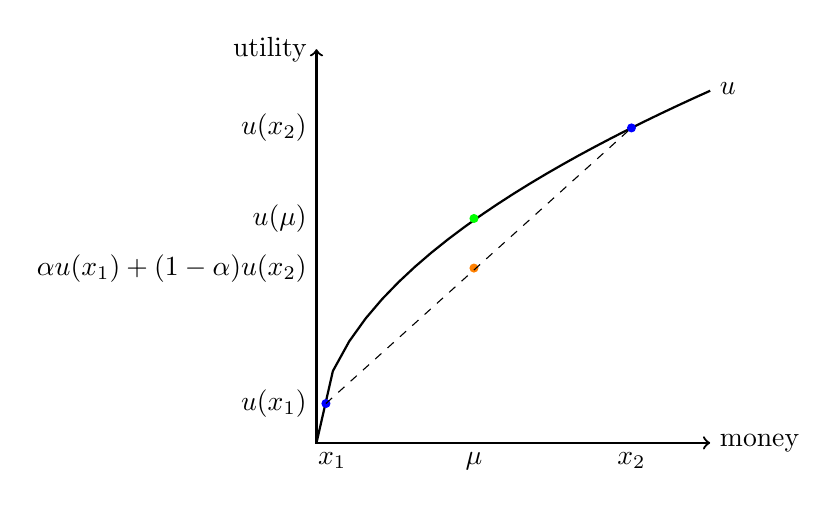
\begin{tikzpicture}
\draw[<->,thick] (5,0) -- (0,0) -- (0,5);
\draw[thick,domain=0:5] plot (\x,{2*sqrt(\x)});
\draw [fill,blue] (0.12,0.5) circle [radius=0.05];
\draw [fill,blue] (4,4) circle [radius=0.05];
\draw [fill,orange] (2,2.22) circle [radius=0.05];
\draw [fill,green] (2,2.85) circle [radius=0.05];
\draw[dashed] (0.12,0.5)--(4,4);
\node[below] at (0.2,0) {$x_1$};
\node[below] at (4,0) {$x_2$};
\node[below] at (2,0) {$\mu$};
\node[left] at (0,0.5) {$u(x_1)$};
\node[left] at (0,4) {$u(x_2)$};
\node[left] at (0,2.22) {$\alpha u(x_1)+(1-\alpha)u(x_2)$};
\node[left] at (0,2.85) {$u(\mu)$};
\node[right] at (5,4.5) {$u$};
\node[right] at (5,0) {money};
\node[left] at (0,5) {utility};
\end{tikzpicture}
\end{figure}
\end{frame}
\end{document}